\chapter{Resumo do projeto}\label{chp:resultadosEsparados}

\section{Enunciado do problema}

Atualmente na medicina, as cirurgias têm o objetivo de causar a mínima agressão ao organismo do paciente, isso implica em um menor tempo de hospitalização; menor incidência de complicações pós-operatórias; menos dor; e recuperação mais rápida \cite{MinInv}. Contudo, entre os diversos desafios de sua realização, a habilidade visual do médico, que envolve a capacidade de localizar e identificar os tecidos sensíveis, é essencial para redução dos danos ao paciente durante um procedimento cirúrgico, nos levando à questão: Como podemos potencializar a visão do médico para aumentar a qualidade dessas operações? 

\begin{figure}[h]
    \centering
    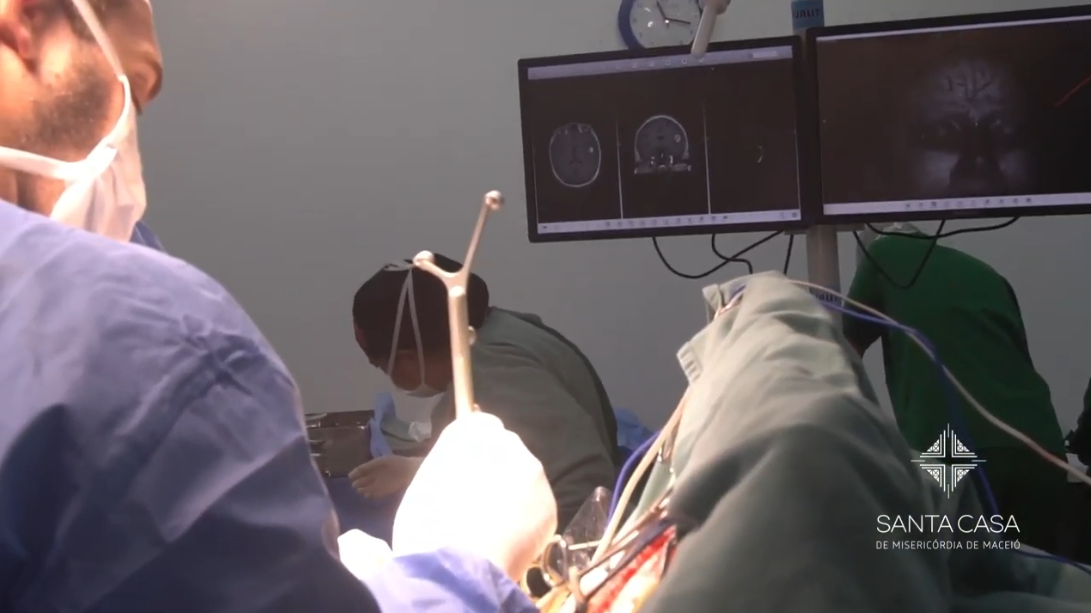
\includegraphics[width=.55\linewidth]{figuras/enunciado.png}
    \caption{Exemplo da utilização de neuronavegador em cirurgia. Fonte: \cite{santacasa}.}
    \label{fig:enunciado}
\end{figure}

Para esse fim, um \textit{software} que informa e assiste o médico em tempo real na operação denota-se como um ótimo meio de aumentar as chances de sucesso dessas cirurgias. Atualmente, esses \textit{softwares} são muito presentes no planejamento e execução das operações, entretanto, toma-se como exemplo os sistemas de neuronavegação, cuja função é permitir visualização, de forma precisa, das estruturas cerebrais do paciente. O neurocirurgião precisa virar a cabeça para ler os monitores e perde o foco na atividade conduzida, colaborando para um maior tempo de operação e favorecendo a exaustão do profissional, de modo que aumente seu potencial de erros durante os procedimentos cirúrgicos (Figura \ref{fig:enunciado}). 

Para isso, a tecnologia de realidade aumentada (\textit{AR}) oferece o potencial de reduzir essas limitações, em razão de que figuras tridimensionais podem sobrepor a visão do médico para facilitar a visualização e a localização dos objetivos da operação enquanto mantém seus olhos direcionados ao paciente \cite{enhancedvision}. O que foi feito nesse projeto é uma pesquisa que envolve visão computacional e computação gráfica no campo do \textit{AR} e uma aplicação para os óculos da empresa \textit{Seiko Epson Corporation\textsuperscript{\textregistered}}, modelo \textit{Moverio BT-350\texttrademark}. Recebendo suporte físico e técnico da equipe do Laboratório Aeronáutico de Tecnologias (Aerotech) da Universidade de São Paulo, esse estudo corrobora com o objetivo do grupo que é desenvolver uma plataforma colaborativa de multi-aplicação neurocirúrgica. 

\section{Objetivo}

Exibir informações e posicionar modelos tridimensionais em uma região do espaço com \textit{AR}, de forma que facilite o acesso do cirurgião à informação durante a neurocirurgia; estudar e registrar a resposta dos equipamentos utilizados no quesito de qualidade gráfica e latência de resposta do sistema. Tudo isso, com o objetivo central de aumentar a proximidade do cirurgião com a tecnologia de \textit{AR} como apoio durante os procedimentos cirúrgicos.

\section{Metodologia}

Consiste na listagem de possíveis soluções, técnicas ou ferramentas; o estudo e a discussão sobre elas, em seguida, sua implementação. Paralelamente a isso, a busca bibliográfica é constantemente realizada com o objetivo de esclarecer dúvidas sobre os meios imaginados e discutidos com o orientador e coorientador. Essa busca enfatiza os resultados encontrados em artigos com o objetivo de caracterizar os prós e contras das diversas opções encontradas. Essa pesquisa de artigos trás uma evolução do discernimento dos assuntos do estado da arte, refletindo em uma noção de funcionamento dos métodos científicos que constrói um novo pesquisador no desenvolvimento dessa iniciação científica.

\section{Breve histórico do projeto}

Desde o início dos trabalhos no projeto, foram experimentados diversos tipos de contato com a elaboração de \textit{softwares} para o sistema operacional \textit{Android} (Figura \ref{fig:sceneform}); testes das ferramentas da documentação dos óculos de realidade aumentada \textit{Moverio BT-350} (Figuras \ref{fig:latinha} e \ref{fig:papercar}); e a elaboração de aplicativos que ilustram o objetivo do \textit{VCranium} \footnote[1]{Nome fantasia atribuído ao \textit{software} em realidade aumentada que projeta as reconstruções virtuais 3D do paciente com o objetivo de trazer uma nova interação para os neurocirurgiões.}
(Figura \ref{fig:vcranium_alpha}). Assim, como foi explicado no relatório parcial da pesquisa, pretendíamos prosseguir o desenvolvimento estabelecendo uma arquitetura composta por computador e óculos para capturar os dados necessários para a projeção em realidade aumentada, os detalhes serão descritos no capítulo das realizações.

\begin{figure}[ht]
\centering
    \begin{subfigure}{0.45\textwidth}
        \centering
        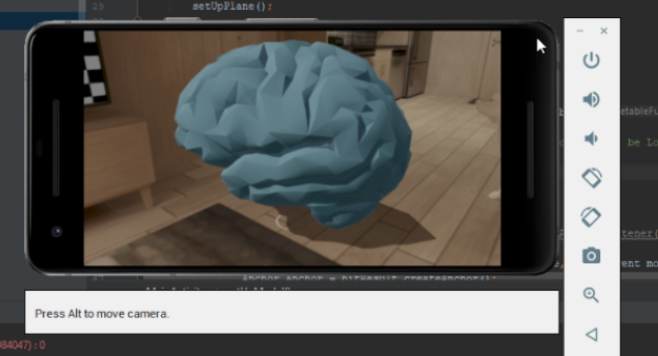
\includegraphics[width=.95\textwidth]{figuras/sceneform.png}
        \caption{Primeiro aplicativo AR para \textit{Android}}
        \label{fig:sceneform}
    \end{subfigure}
    \begin{subfigure}{0.45\textwidth}
        \centering
        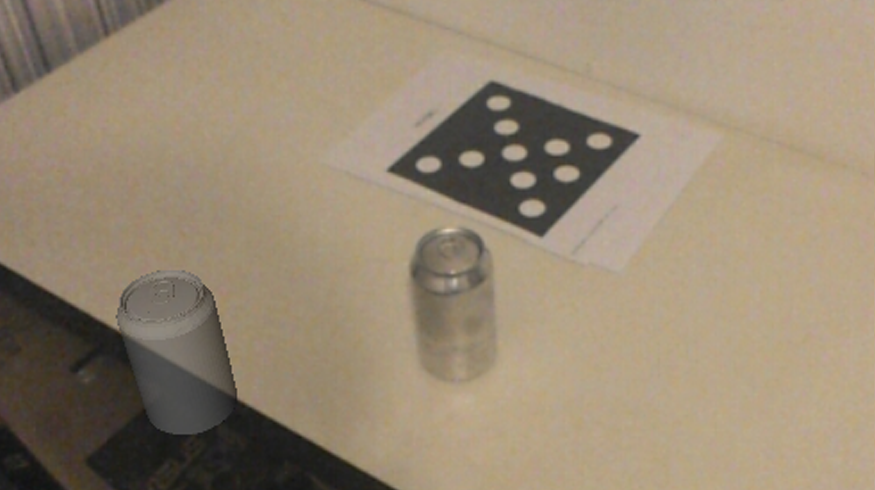
\includegraphics[width=.95\linewidth]{figuras/Latinha-errada.png}
        \caption{Tentativa de calibração do \textit{Moverio}}
        \label{fig:latinha}
    \end{subfigure}
    \begin{subfigure}{0.45\textwidth}
        \centering
        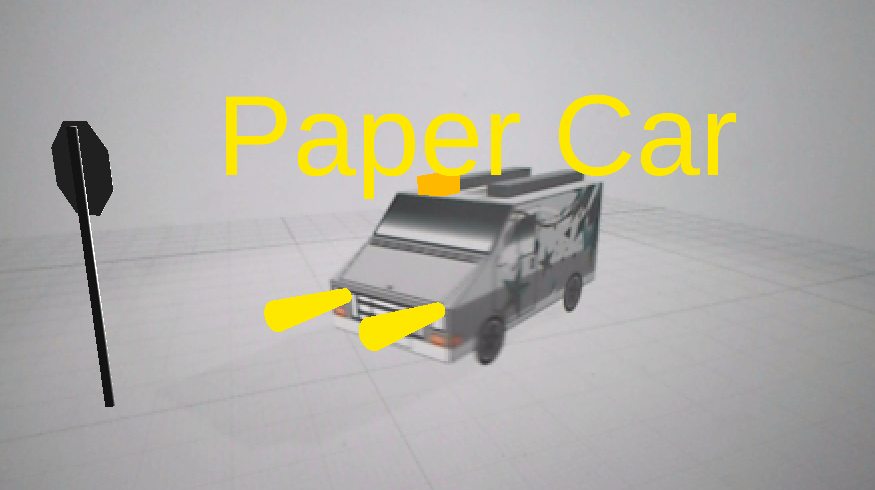
\includegraphics[width=.95\textwidth]{figuras/PaperCarAR.png}
        \caption{Aplicativo fornecido pela \textit{EPSON}}
        \label{fig:papercar}
    \end{subfigure}
    \begin{subfigure}{0.45\textwidth}
        \centering
        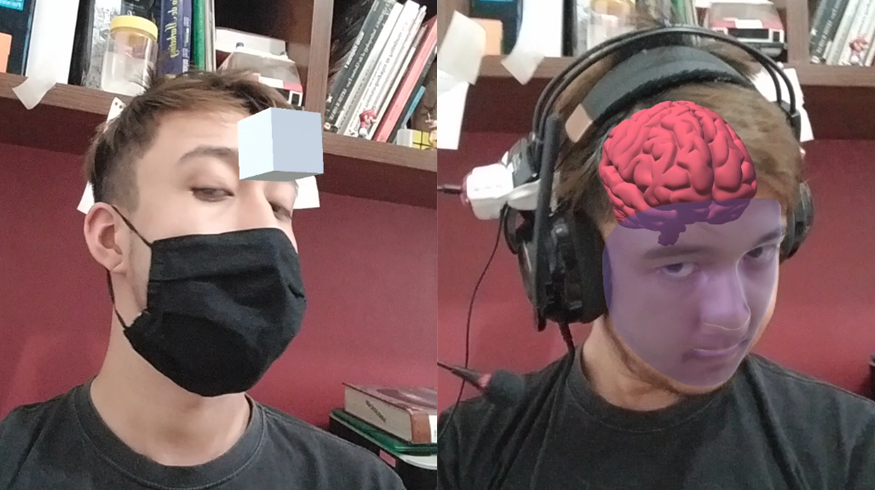
\includegraphics[width=.95\linewidth]{figuras/VCranium.png}
        \caption{Primeira versão do \textit{VCranium}}
        \label{fig:vcranium_alpha}
    \end{subfigure}
    \caption{Histórico de realizações da pesquisa até a primeira entrega parcial. Fonte: Autor.}
    \label{fig:historico}
\end{figure}


